\documentclass[10pt,pdf,utf8,aspectratio=169,xcolor=dvipsnames,x11names,center]{beamer}

\usepackage[T2A]{fontenc}
\usepackage[english,russian]{babel}
\usepackage[utf8]{inputenc}

\usepackage{pgfpages}
%%\setbeameroption{show notes}
%%\setbeameroption{show notes on second screen=right}

\usepackage{dirtytalk}

\usepackage{listings}

\definecolor{light-gray}{gray}{0.95}
\lstset{
language=Python,                             % Code langugage
basicstyle=\small,                   % Code font, Examples: \footnotesize, \ttfamily
keywordstyle=\color{JungleGreen},        % Keywords font ('*' = uppercase)
commentstyle=\color{gray},              % Comments font
numbers=left,                           % Line nums position
numberstyle=\tiny,                      % Line-numbers fonts
stringstyle=\color{BrickRed},          %
stepnumber=1,                           % Step between two line-numbers
numbersep=5pt,                          % How far are line-numbers from code
backgroundcolor=\color{light-gray},     % Choose background color
frame=lines,                            % A frame around the code
tabsize=4,                              % Default tab size
captionpos=b,                           % Caption-position = bottom
breaklines=true,                        % Automatic line breaking?
breakatwhitespace=false,                % Automatic breaks only at whitespace?
showspaces=false,                       % Don't make spaces visible
showstringspaces=false,                 % Don't show spaces in string literals 
showtabs=false,                         % Don't make tabs visible
}

\title[Remote]{\Large{Про процессы, и потоки, и Python}}

\author[]{\Large{Стас Рудаков}\\\small{stas@garage22.net}}

\date{Minsk Python Meetup\\August 2018}

\begin{document}

\begin{frame}
  \titlepage
\end{frame}

\begin{frame}
  \begin{figure}
    \includegraphics[scale=0.05]{DataRobot_Logo}
  \end{figure}
\end{frame}

\begin{frame}[fragile,label=src]
  \begin{lstlisting}
import logging
from multiprocessing import Process
from threading import Thread
import time

logging.basicConfig(level='INFO')

def foobar(identity):
    for i in range(1000):
        logging.info('I am {}'.format(identity))
        time.sleep(0.001)

t = Thread(target=foobar, args=('thread',))
p = Process(target=foobar, args=('process',))

t.start()
p.start()

t.join()
logging.info('thread joined')
p.join()
logging.info('process joined')
  \end{lstlisting}
\end{frame}

\begin{frame}[fragile]
  \frametitle{Запустим}
  \begin{lstlisting}[language=bash]
python3 /src/example.py
  \end{lstlisting}
  \begin{lstlisting}[language={}]
[...]
INFO:root:I am thread
INFO:root:I am process
INFO:root:I am thread
INFO:root:I am process
INFO:root:I am thread
INFO:root:I am process
INFO:root:I am thread
INFO:root:I am process
INFO:root:I am thread
INFO:root:I am process
INFO:root:thread joined
INFO:root:I am process
INFO:root:I am process
INFO:root:I am process
INFO:root:I am process
INFO:root:process joined
  \end{lstlisting}
\end{frame}

\begin{frame}[fragile]
  \frametitle{Запустим еще несколько раз... упс}
  \begin{lstlisting}[language=bash]
for i in $(seq 100); do echo attempt $i; python3 /src/example.py; done
  \end{lstlisting}
  \begin{lstlisting}[language={}]
[...]
attempt 12
[...]
INFO:root:I am thread
INFO:root:I am thread
INFO:root:I am thread
INFO:root:I am thread
INFO:root:I am thread
INFO:root:I am thread
INFO:root:I am thread
INFO:root:I am thread
INFO:root:I am thread
INFO:root:I am thread
INFO:root:I am thread
INFO:root:thread joined
  \end{lstlisting}
\end{frame}

\begin{frame}[fragile]
  \frametitle{Для истории: подготовка окружения}
  \begin{lstlisting}[language={}]
$ docker run -it -v `pwd`:/src --privileged ubuntu:18.04
root@06f40dc80b14:/# apt update
[...]
root@06f40dc80b14:/# apt install python3
[...]
  \end{lstlisting}
\end{frame}

\begin{frame}[fragile]
  \frametitle{Что вообще происходит?}
  \begin{lstlisting}[language={}]
root@e681a8ffef5b:/# ps -ef --forest
UID    PID  PPID  C STIME TTY        TIME CMD
root   626     0  0 05:49 pts/1  00:00:00 bash
root   638   626  0 05:49 pts/1  00:00:00  \_ ps -ef --forest
root     1     0  0 Aug15 pts/0  00:00:00 /bin/bash
root   623     1  0 05:43 pts/0  00:00:00 python3 /src/example.py
root   625   623  0 05:43 pts/0  00:00:00  \_ python3 /src/example.py
  \end{lstlisting}
\end{frame}

\againframe{src}

\begin{frame}[fragile]
  \frametitle{Нам нужен дебаггер!}
  \begin{lstlisting}[language={}]
root@06f40dc80b14:/# apt install gdb
[...]
  \end{lstlisting}
\end{frame}

\begin{frame}[fragile]
  \frametitle{Подебажим}
  \begin{lstlisting}[language=bash]
gdb -p 625
  \end{lstlisting}
  \begin{lstlisting}[language={}]
[...]
For help, type "help".
Type "apropos word" to search for commands related to "word".
Attaching to process 625
Reading symbols from /usr/bin/python3.6...(no debugging symbols found)...done.
[...]
(gdb)
  \end{lstlisting}
\end{frame}

\begin{frame}[fragile]
  \begin{lstlisting}[language={}]
(gdb) bt
#0  0x00007f0cbc6a66d6 in futex_abstimed_wait_cancelable (private=0, 
    abstime=0x0, expected=0, futex_word=0x15b82e0)
    at ../sysdeps/unix/sysv/linux/futex-internal.h:205
#1  do_futex_wait (sem=sem@entry=0x15b82e0, abstime=0x0)
    at sem_waitcommon.c:111
#2  0x00007f0cbc6a67c8 in __new_sem_wait_slow (sem=0x15b82e0, abstime=0x0)
    at sem_waitcommon.c:181
#3  0x000000000043f0a8 in PyThread_acquire_lock_timed ()
#4  0x000000000058fbfd in ?? ()
#5  0x00000000004c549b in _PyCFunction_FastCallKeywords ()
#6  0x000000000054ffe4 in ?? ()
#7  0x00000000005546cf in _PyEval_EvalFrameDefault ()
#8  0x000000000054f0e8 in ?? ()
#9  0x0000000000550116 in ?? ()
#10 0x00000000005546cf in _PyEval_EvalFrameDefault ()
#11 0x000000000054f0e8 in ?? ()
#12 0x0000000000550116 in ?? ()
---Type <return> to continue, or q <return> to quit---
  \end{lstlisting}
\end{frame}

\begin{frame}[fragile]
  \frametitle{Символизируем}
  \begin{lstlisting}[language={}]
root@06f40dc80b14:/# apt install python3-dbg
[...]
  \end{lstlisting}
\end{frame}

\begin{frame}[fragile]
  \frametitle{Подебажим с символами}
  \begin{lstlisting}[language=bash]
gdb -p 625
  \end{lstlisting}
  \begin{lstlisting}[language={}]
[...]
For help, type "help".
Type "apropos word" to search for commands related to "word".
Attaching to process 625
Reading symbols from /usr/bin/python3.6...Reading symbols from /usr/lib/debug/.build-id/2c/3972a143bed2ede030627a64ce934ea4398f18.debug...done.
done.
[...]
(gdb)
  \end{lstlisting}
\end{frame}

\begin{frame}[fragile]
  \begin{lstlisting}[language={}]
(gdb) bt
#0  0x00007f0cbc6a66d6 in futex_abstimed_wait_cancelable (private=0, abstime=0x0, 
    expected=0, futex_word=0x15b82e0) at ../sysdeps/unix/sysv/linux/futex-internal.h:205
#1  do_futex_wait (sem=sem@entry=0x15b82e0, abstime=0x0) at sem_waitcommon.c:111
#2  0x00007f0cbc6a67c8 in __new_sem_wait_slow (sem=sem@entry=0x15b82e0, abstime=0x0)
    at sem_waitcommon.c:181
#3  0x00007f0cbc6a6839 in __new_sem_wait (sem=sem@entry=0x15b82e0) at sem_wait.c:42
#4  0x000000000043f0a8 in PyThread_acquire_lock_timed (lock=lock@entry=0x15b82e0, 
    microseconds=microseconds@entry=-1000000, intr_flag=intr_flag@entry=1)
    at ../Python/thread_pthread.h:354
#5  0x000000000058fbfd in acquire_timed (timeout=-1000000000, lock=0x15b82e0)
    at ../Modules/_threadmodule.c:68
  \end{lstlisting}
\end{frame}

\begin{frame}[fragile]
  \begin{lstlisting}[language={}]
#6  rlock_acquire (self=0x7f0cbc9c4660, args=<optimized out>, kwds=<optimized out>)
    at ../Modules/_threadmodule.c:314
#7  0x00000000004c549b in _PyCFunction_FastCallDict (kwargs=0x0, nargs=139692680693344, 
    args=0x7f0cbb5ec870, 
    func_obj=<built-in method acquire of _thread.RLock object at remote 0x7f0cbc9c4660>)
    at ../Objects/methodobject.c:231
#8  _PyCFunction_FastCallKeywords (
    func=func@entry=<built-in method acquire of _thread.RLock object at remote 0x7f0cbc9c4660>, stack=stack@entry=0x7f0cbb5ec870, nargs=nargs@entry=0, kwnames=kwnames@entry=0x0)
    at ../Objects/methodobject.c:294
#9  0x000000000054ffe4 in call_function (pp_stack=pp_stack@entry=0x7ffeb109d4a8, 
    oparg=<optimized out>, kwnames=kwnames@entry=0x0) at ../Python/ceval.c:4824
#10 0x00000000005546cf in _PyEval_EvalFrameDefault (f=<optimized out>, 
    throwflag=<optimized out>) at ../Python/ceval.c:3322
  \end{lstlisting}
\end{frame}

\begin{frame}[fragile]
  \frametitle{Жемчужина}
  \begin{lstlisting}[language={}]
#11 0x000000000054f0e8 in PyEval_EvalFrameEx (throwflag=0, 
    f=Frame 0x7f0cbb5ec6e8, for file /usr/lib/python3.6/logging/__init__.py, line 812, in acquire (self=<StreamHandler(filters=[], _name=None, level=0, formatter=<Formatter(_style=<PercentStyle(_fmt='%(levelname)s:%(name)s:%(message)s') at remote 0x7f0cbc962be0>, _fmt='%(levelname)s:%(name)s:%(message)s', datefmt=None) at remote 0x7f0cbc962ba8>, lock=<_thread.RLock at remote 0x7f0cbc9c4660>, stream=<_io.TextIOWrapper at remote 0x7f0cbca7b708>) at remote 0x7f0cbc962b70>)) at ../Python/ceval.c:753
---Type <return> to continue, or q <return> to quit---
  \end{lstlisting}
\end{frame}

\begin{frame}[fragile]
  \frametitle{Используем Python extensions}
  \begin{lstlisting}[language={}]
(gdb) py-bt
Traceback (most recent call first):
  <built-in method acquire of _thread.RLock object at remote 0x7f0cbc9c4660>
  File "/usr/lib/python3.6/logging/__init__.py", line 812, in acquire
    self.lock.acquire()
  File "/usr/lib/python3.6/logging/__init__.py", line 861, in handle
    self.acquire()
  File "/usr/lib/python3.6/logging/__init__.py", line 1514, in callHandlers
    hdlr.handle(record)
  File "/usr/lib/python3.6/logging/__init__.py", line 1452, in handle
    self.callHandlers(record)
  File "/usr/lib/python3.6/logging/__init__.py", line 1442, in _log
    self.handle(record)
  File "/usr/lib/python3.6/logging/__init__.py", line 1306, in info
    self._log(INFO, msg, args, **kwargs)
  File "/usr/lib/python3.6/logging/__init__.py", line 1900, in info
    root.info(msg, *args, **kwargs)
  \end{lstlisting}
\end{frame}

\begin{frame}[fragile]
  \frametitle{Используем Python extensions (немного терпения)}
  \begin{lstlisting}[language={}]
  File "/src/example.py", line 9, in foobar
    logging.info('I am {}'.format(identity))
  File "/usr/lib/python3.6/multiprocessing/process.py", line 93, in run
    self._target(*self._args, **self._kwargs)
  File "/usr/lib/python3.6/multiprocessing/process.py", line 258, in _bootstrap
    self.run()
  File "/usr/lib/python3.6/multiprocessing/popen_fork.py", line 73, in _launch
    code = process_obj._bootstrap()
  File "/usr/lib/python3.6/multiprocessing/popen_fork.py", line 19, in __init__
    self._launch(process_obj)
  File "/usr/lib/python3.6/multiprocessing/context.py", line 277, in _Popen
    return Popen(process_obj)
  File "/usr/lib/python3.6/multiprocessing/context.py", line 223, in _Popen
    return _default_context.get_context().Process._Popen(process_obj)
  \end{lstlisting}
\end{frame}

\begin{frame}[fragile]
  \frametitle{Используем Python extensions (вот оно)}
  \begin{lstlisting}[language={}]
  File "/usr/lib/python3.6/multiprocessing/process.py", line 105, in start
    self._popen = self._Popen(self)
  File "/src/example.py", line 20, in main
    p.start()
  File "/src/example.py", line 30, in <module>
    main()
  \end{lstlisting}
\end{frame}

\begin{frame}[fragile]
  \begin{lstlisting}[caption=logging/\_\_init\_\_.py\#L851-L867]
class Handler(Filterer):
    [...]
    def handle(self, record):
        """
        Conditionally emit the specified logging record.
        Emission depends on filters which may have been added to the handler.
        Wrap the actual emission of the record with acquisition/release of
        the I/O thread lock. Returns whether the filter passed the record for
        emission.
        """
        rv = self.filter(record)
        if rv:
            self.acquire()
            try:
                self.emit(record)
            finally:
                self.release()
        return rv
  \end{lstlisting}
\end{frame}

\againframe{src}

\begin{frame}
  \begin{figure}
    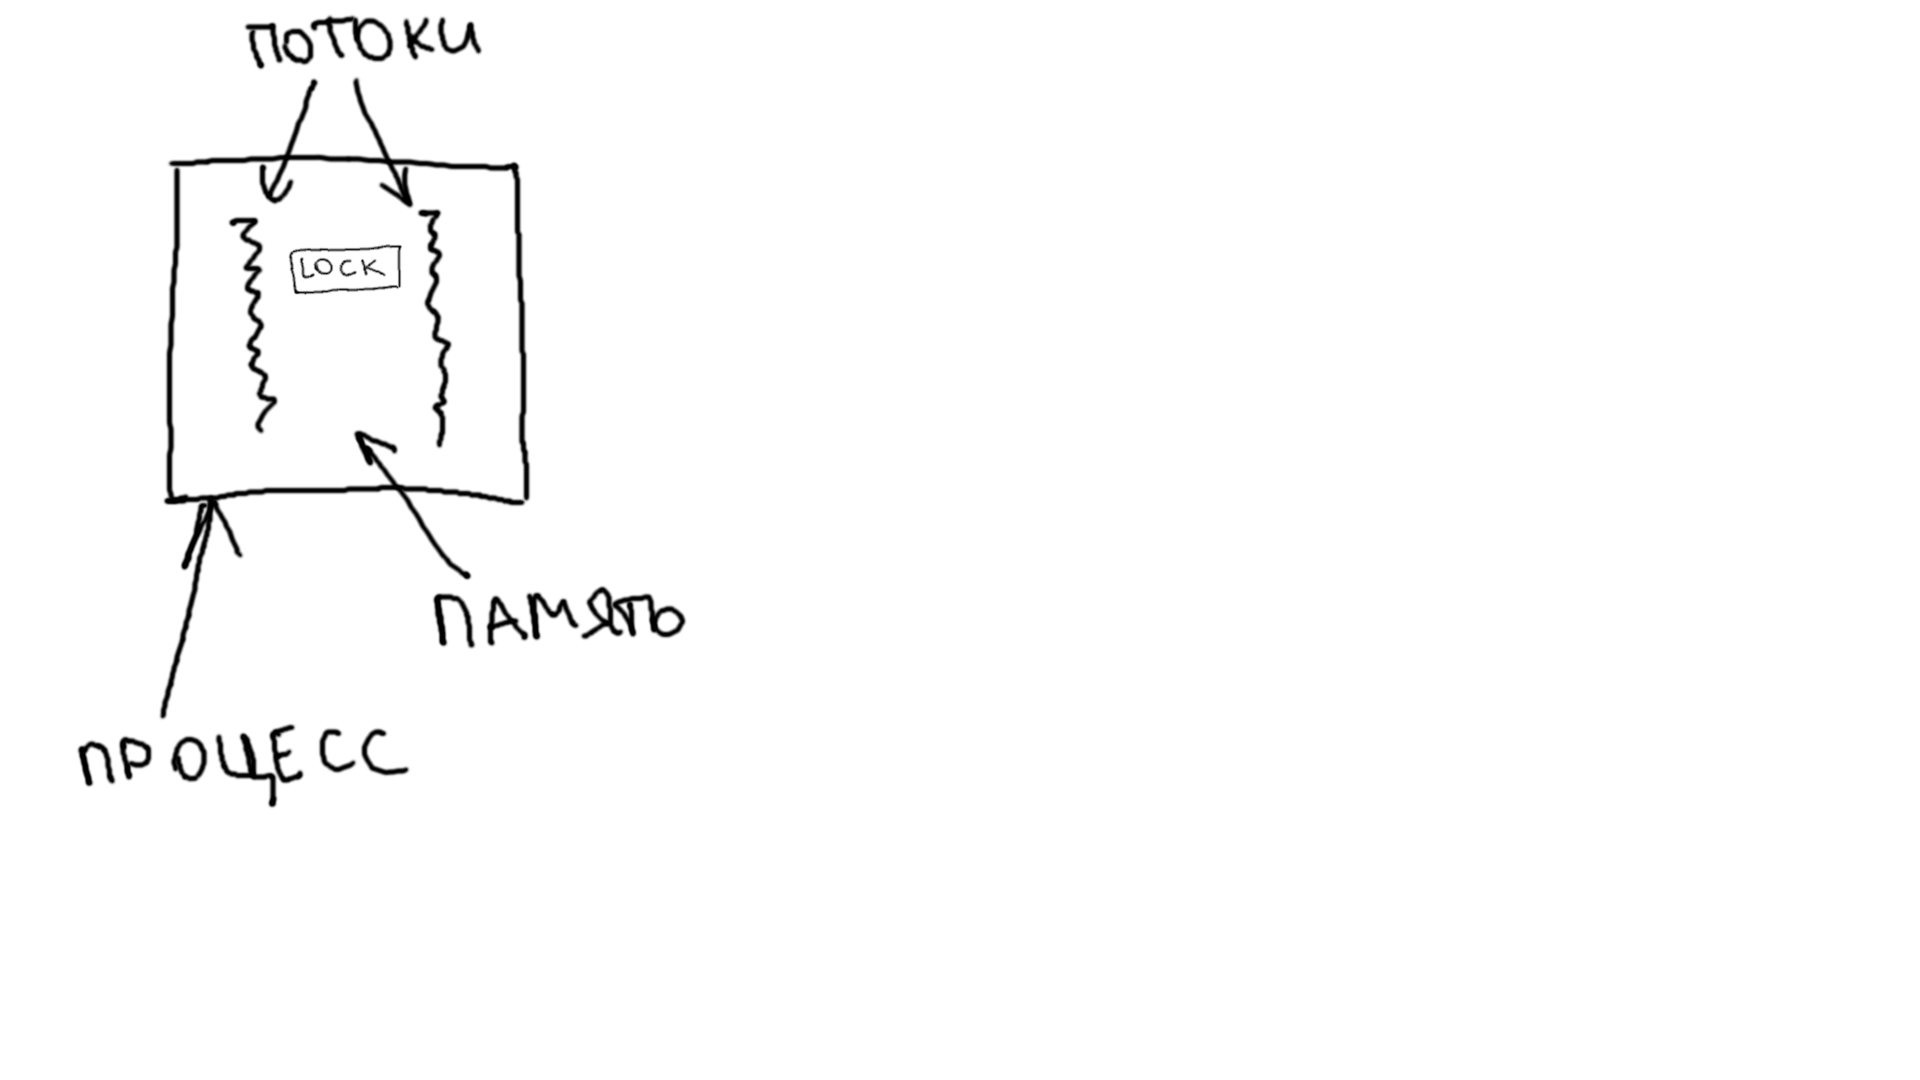
\includegraphics[scale=0.8]{diagrams/single_process}
  \end{figure}
\end{frame}

\begin{frame}
  \begin{figure}
    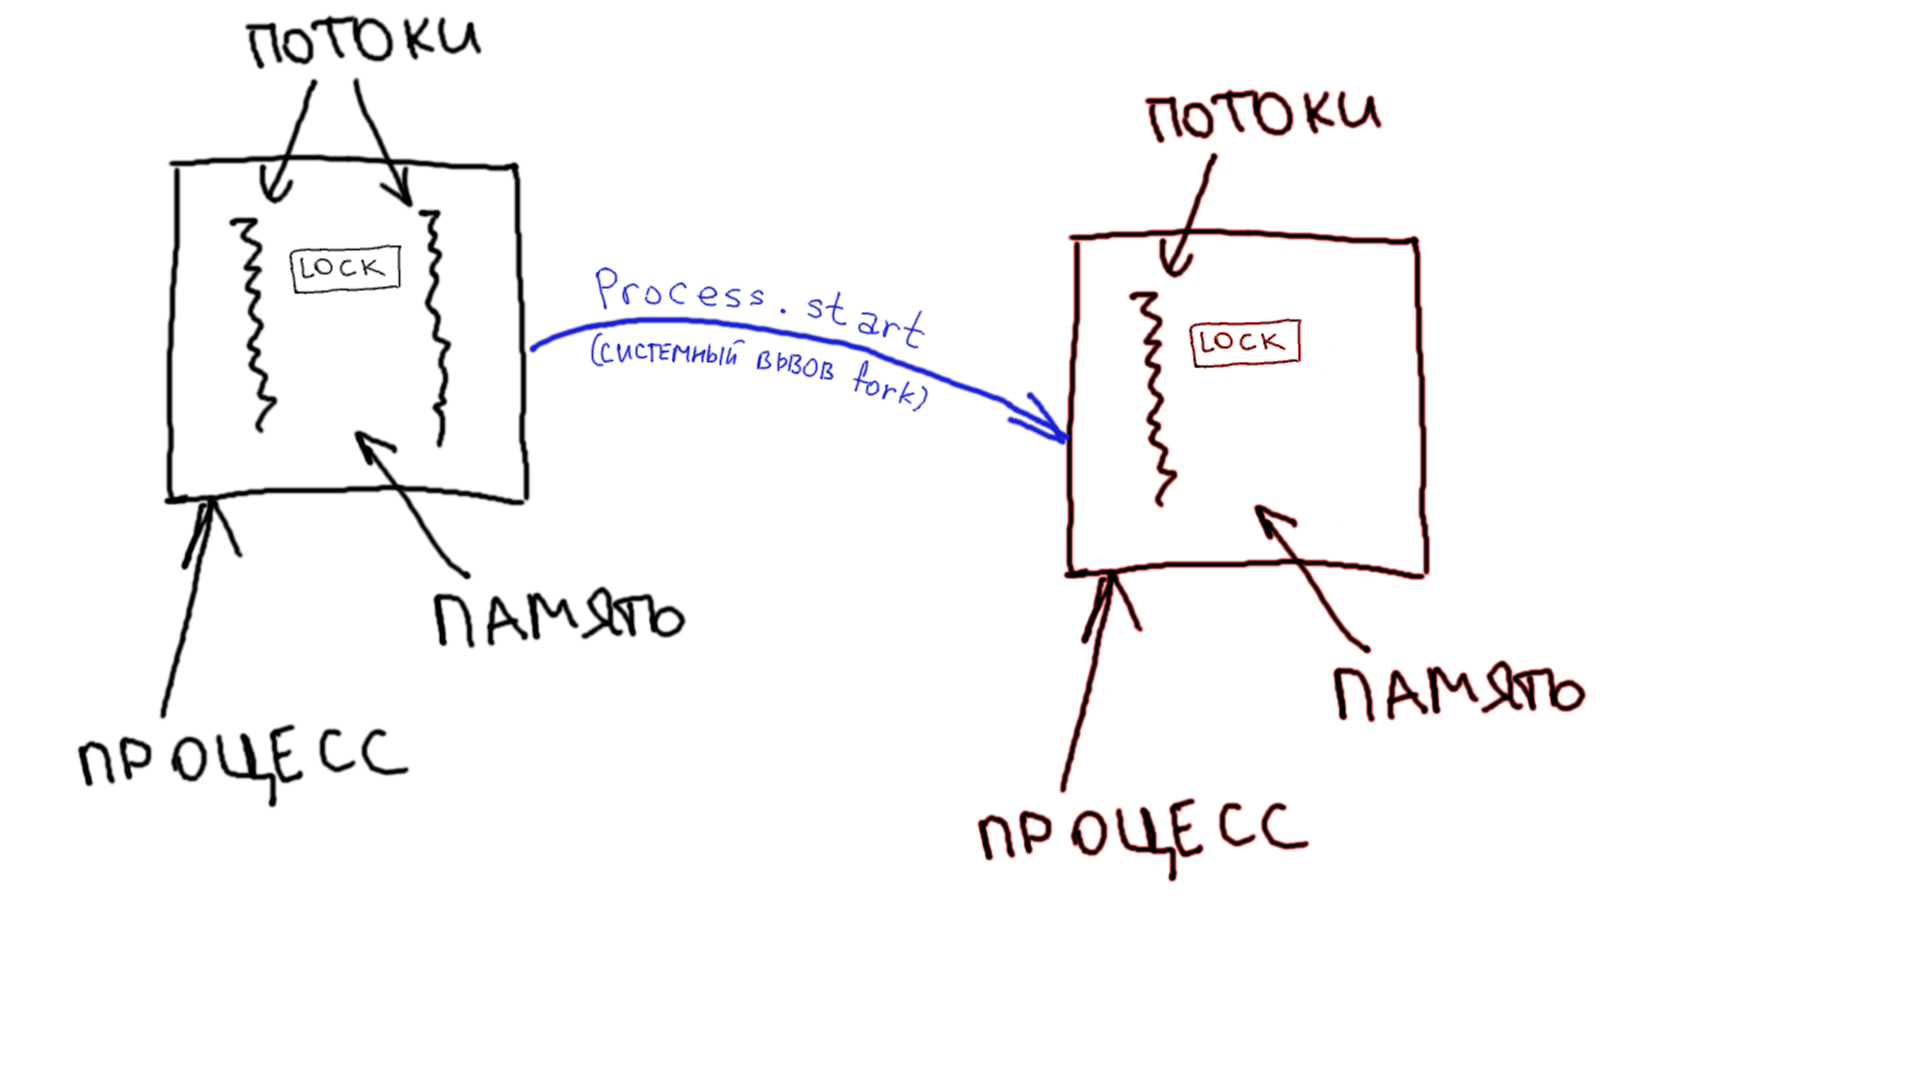
\includegraphics[scale=0.8]{diagrams/fork}
  \end{figure}
\end{frame}

\begin{frame}
  \begin{figure}
    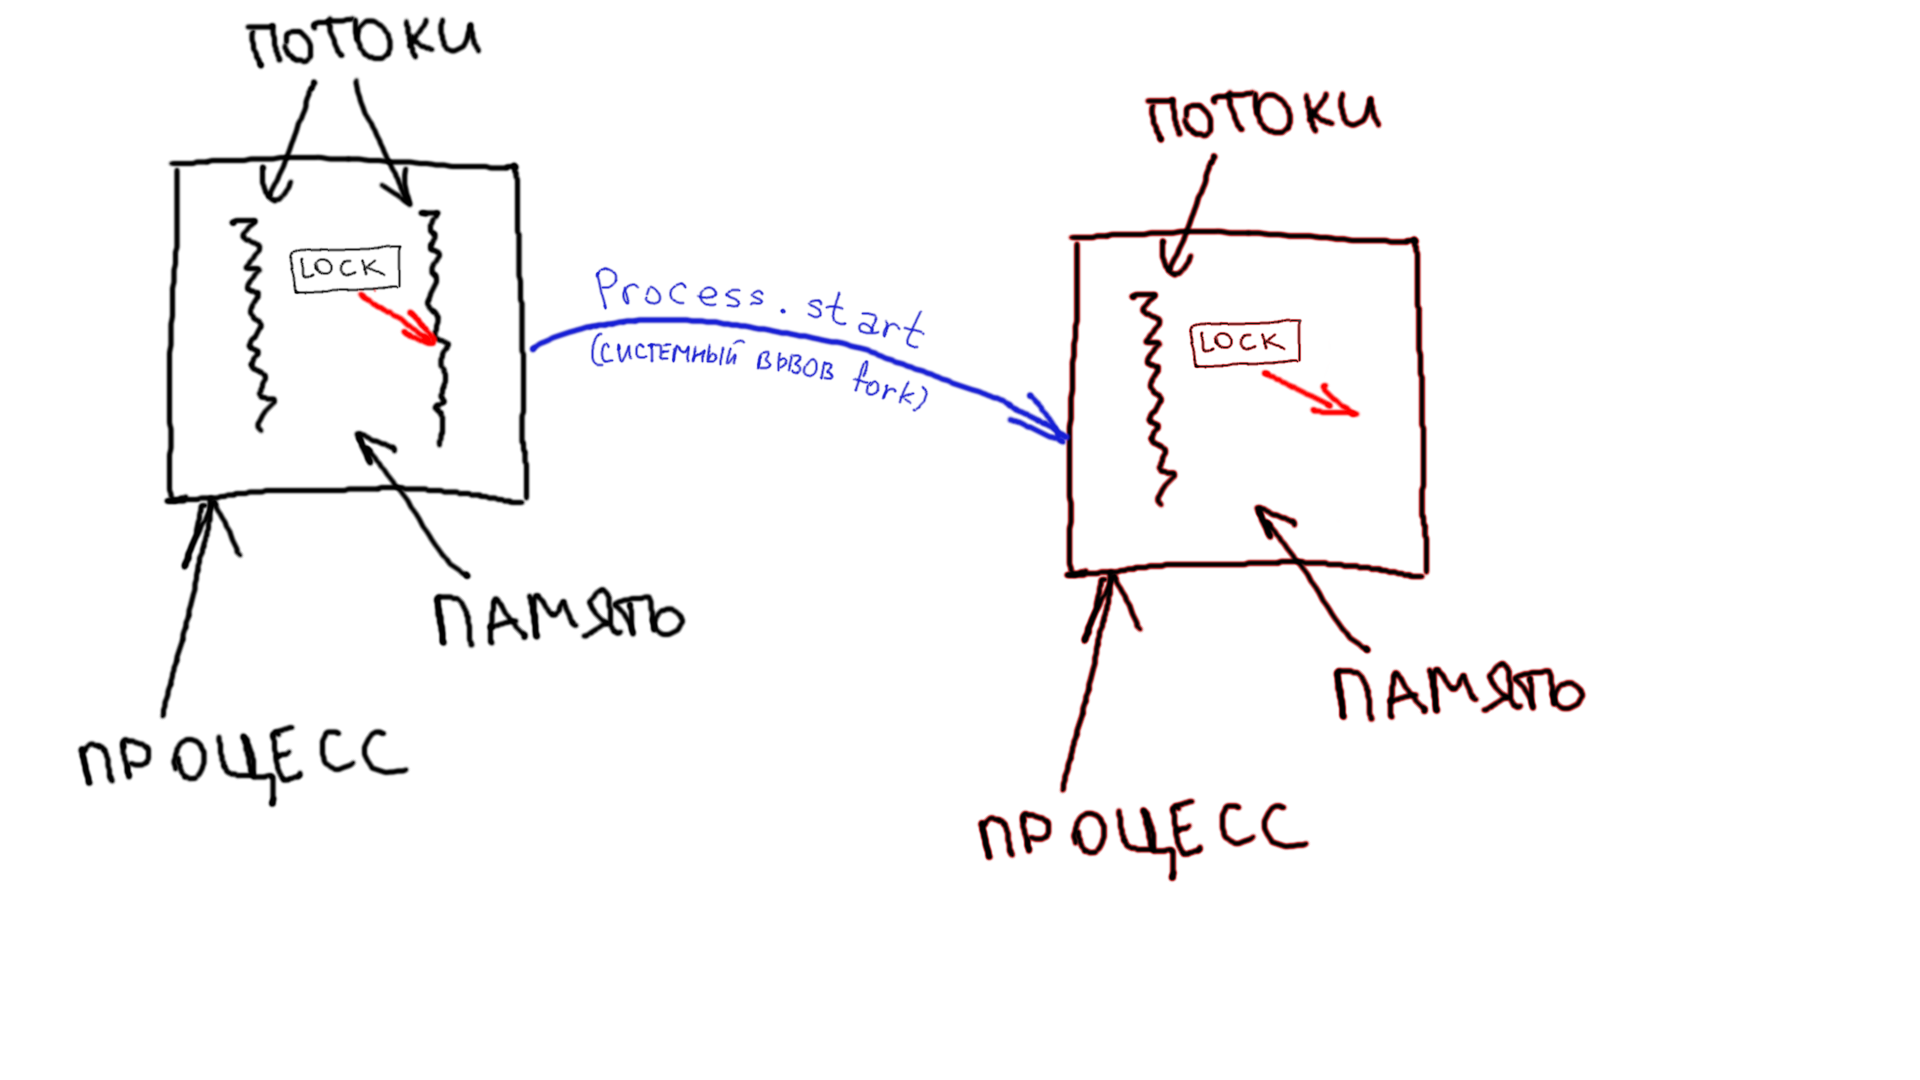
\includegraphics[scale=0.8]{diagrams/locked}
  \end{figure}
\end{frame}

\begin{frame}
  \frametitle{Но как это касается лично меня?}
  Библиотека, которую вы используете,\\может запускать потоки под капотом
  \begin{itemize}
  \item pymongo
  \item raven (sentry client)
  \end{itemize}
\end{frame}

\begin{frame}[fragile]
  \frametitle{Окей... но что делать?}
  \begin{enumerate}
  \item Форкаться как можно раньше
    \begin{lstlisting}
process.start()
thread.start()
    \end{lstlisting}
    \pause
  \item Не использовать потоки в своем коде (заменить \texttt{threading} на \texttt{multiprocessing})
    \pause
  \item Разблокировать все lock'и после форка
    \begin{lstlisting}
def process_target(identity):
    logging._releaseLock()
    return foobar(identity)
        
process = Process(target=process_target, args=('process',))
process.start()    
    \end{lstlisting}
  \end{enumerate}
\end{frame}

\begin{frame}
  \frametitle{Что почитать?}
  \begin{itemize}
  \item \texttt{man 2 fork}
  \item \url{https://wiki.python.org/moin/DebuggingWithGdb}
  \item \url{https://devguide.python.org/gdb/}
  \end{itemize}
\end{frame}

\begin{frame}
    \begin{block}{Стас Рудаков}
    \par \url{mailto:stas@garage22.net}
    \par \url{http://staaas.net/talks.html}
    \end{block}
\end{frame}

\end{document}
